\documentclass[class=report, crop=false]{standalone}
\usepackage[subpreambles=true]{standalone}

\begin{document}
    \section{Resultatet}
    Efter kørslen af programmerne, kunne vi sammenligne resultaterne som kan ses herunder. Det ses at C\# programmet køre betydeligt hurtigere end Python programmet.\\
    Resultatets middelværdi lå meget højere i Python, som vi havde forventet. Men udover dette er differencen også en del højere som vi ikke havde forventet. Ved at skrive alle gennemsnitsværdierne ud istedet for middelværdien kunne vi plotte de to programmersom kan ses på Figur \ref{fig:SpeedPlot}. Dette gav et tydeligt indblik i stabiliteten af de to sprog, som viser at Python køre meget mere ustabilt også. 
    
    \begin{tcolorbox}
        \text{C\#: } \[ 311,2 \text{ ns} \pm 13,1  \]
    \end{tcolorbox}
    \begin{tcolorbox}
        \text{Python: } \[ 3312,1 \text{ ns} \pm 88,9  \]
    \end{tcolorbox}

    \begin{tcolorbox}
        \begin{figure}[H]
            \centering
            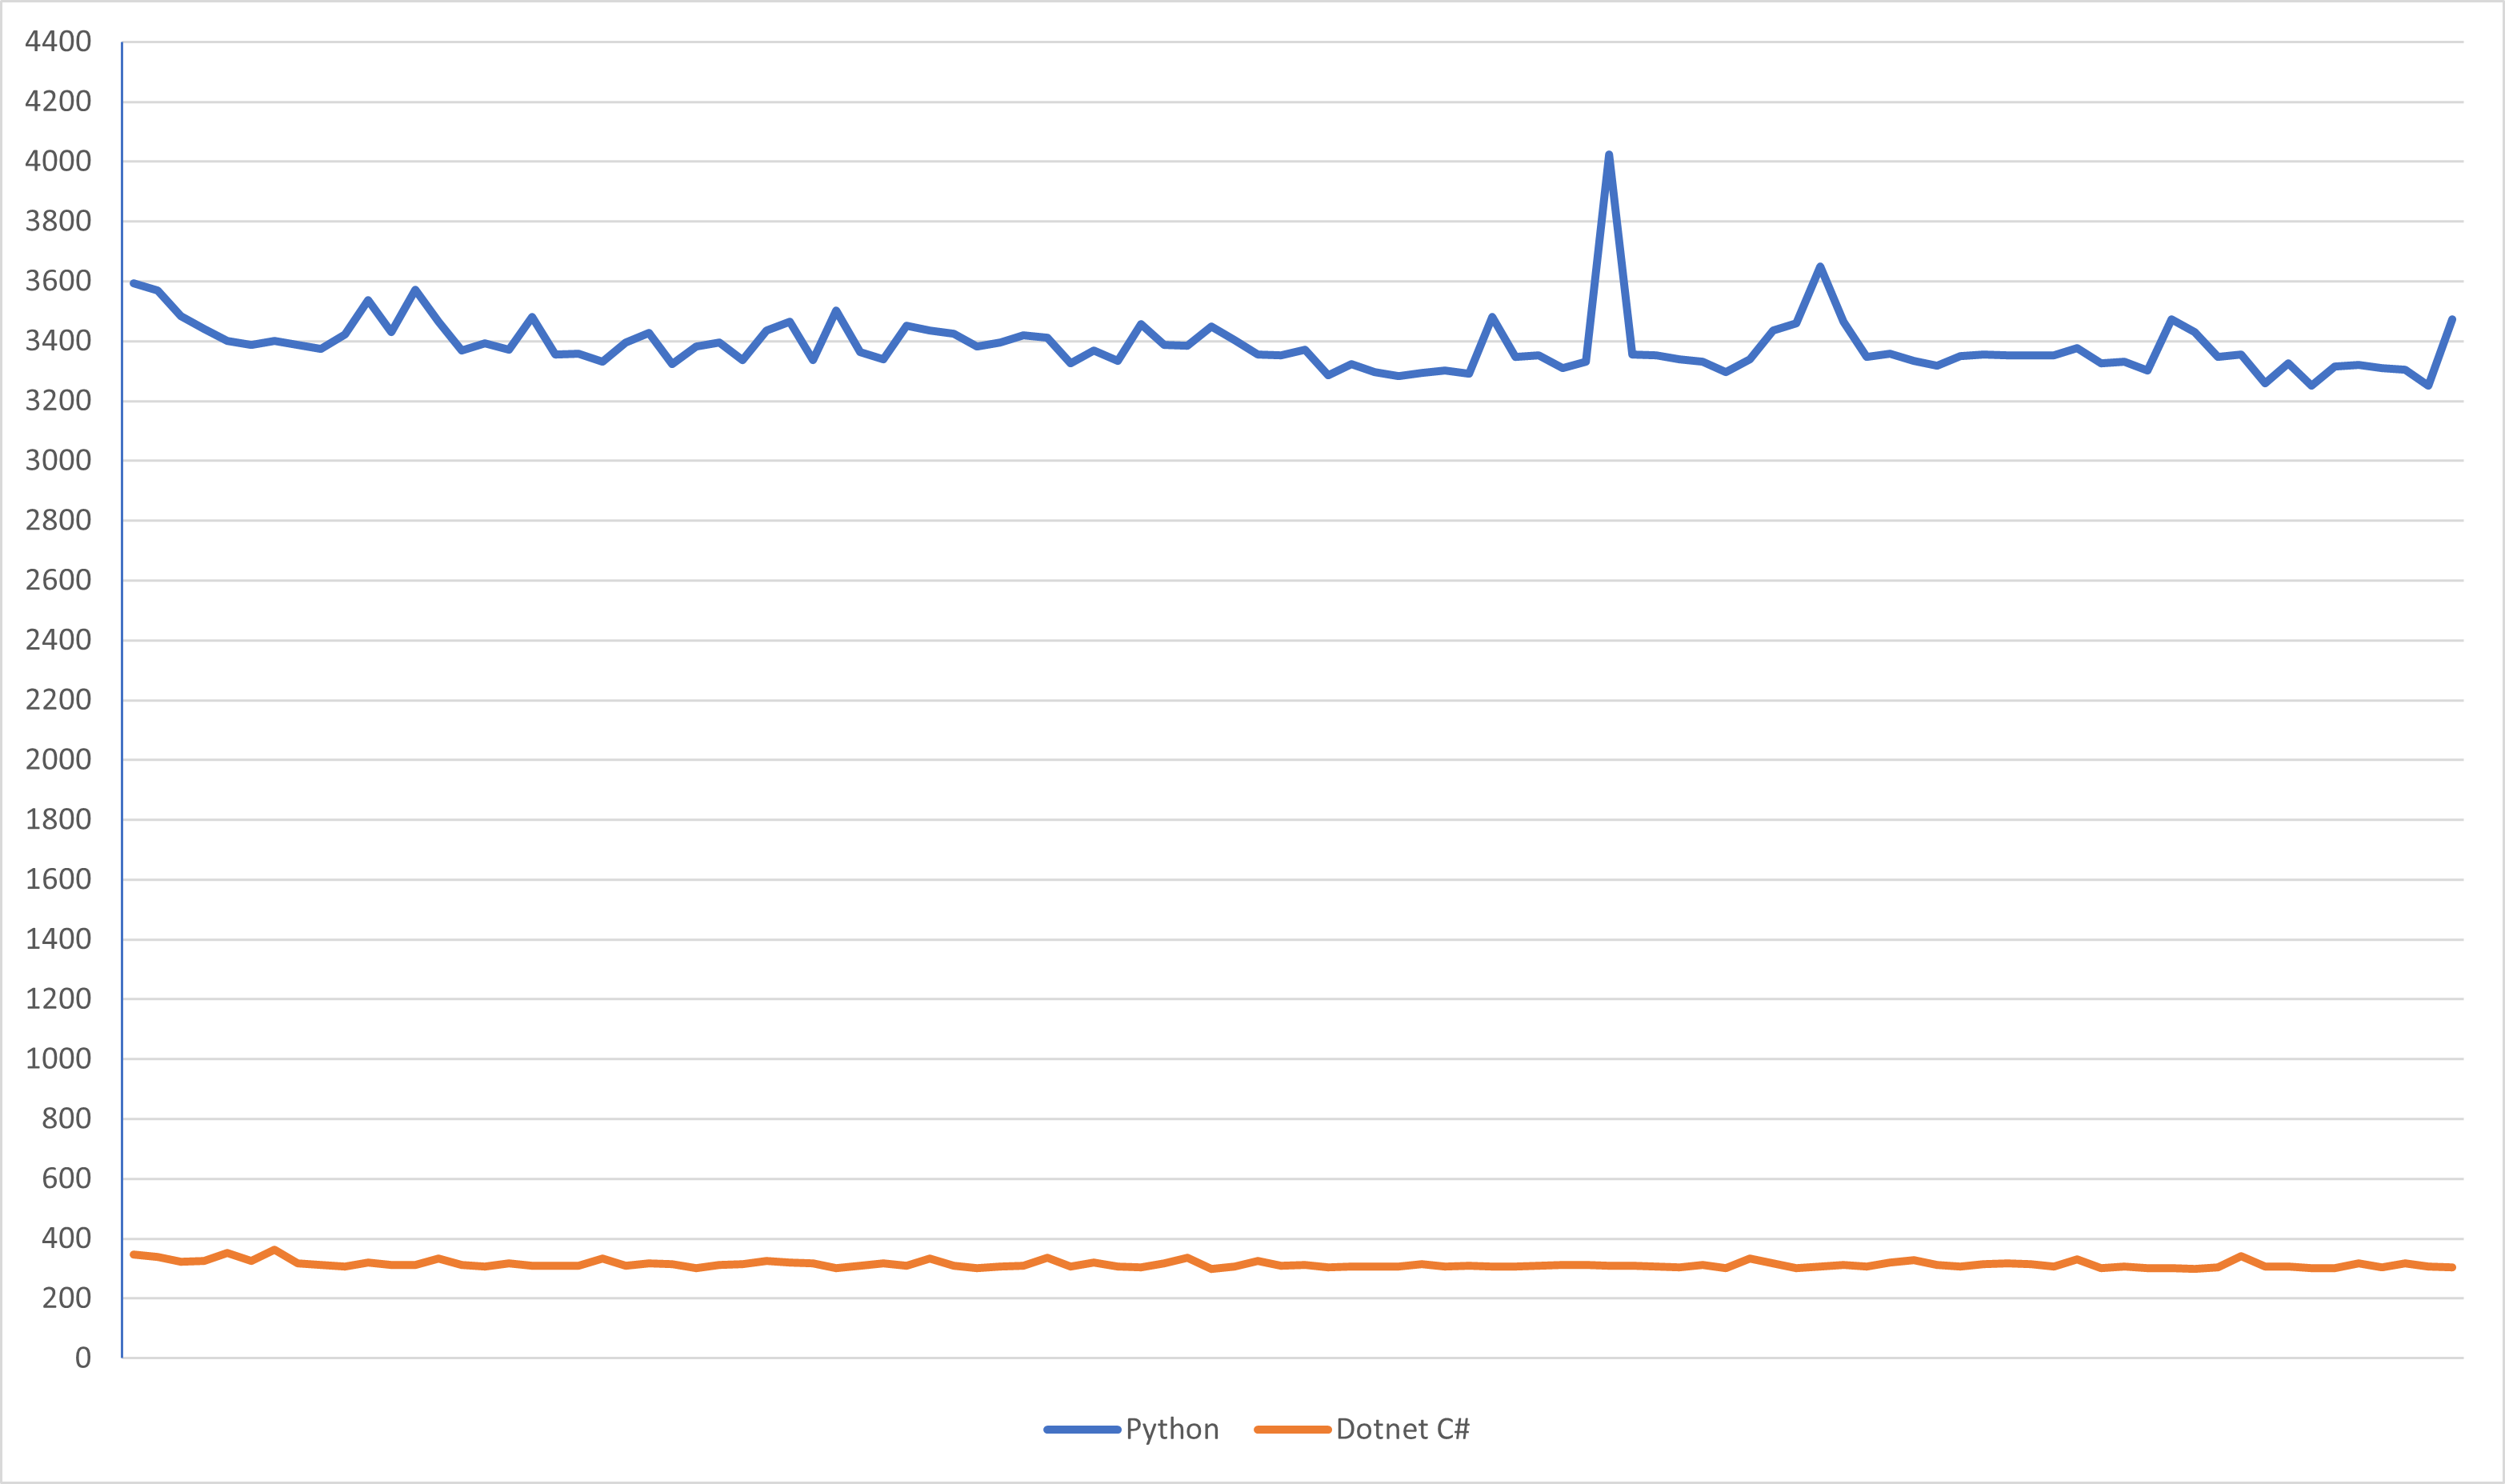
\includegraphics[width=\textwidth]{SpeedPlot.png}
            \caption{Plot af hastighed på Insertion Sort}
            \label{fig:SpeedPlot}
        \end{figure}
    \end{tcolorbox}

\end{document}